% Chapter Template

\chapter{Steady State Analysis}

\label{Chapter2}

\lhead{Chapter 2. \emph{Steady State Response Analysis Using Frequency Response}} 

If one is interested in the steady state response only, an easier route would to use the frequency response of the system.
\section{Frequency Response }
    Suppose the input to a circuit is characterized by the following Fourier series,
    \begin{align*}
       V_{i} = V_{i, dc} + \sum C_n e^{j\omega nt} 
    \end{align*}
    The output current can be characterized by a Fourier series like the following,
    \begin{align*}
       I_{o} = I_{o, dc} + \sum C_{n}^{\prime}  e^{j\omega nt} 
    \end{align*}
   What we are interested in is a function of the angular frequency which can relate $C_n$ and $C_{n}^\prime$
   \begin{align*}
       C_n ^\prime = H\brak{j\omega} \cdot C_n
   \end{align*}
   The function H, commonly known as the \texttt{transfer function}, can be calculated easily by treating the quantities $C_n e^{j\omega nt}$ as the input voltage phasor and $C_n^\prime e^{j\omega nt}$ as the corresponding output phasor. 
   \begin{align*}
       \vec{I}_{o,n} = H\brak{jw} \cdot \vec{V}_{i,n}
   \end{align*}
\section{Calculating the transfer function}
   \begin{figure}[!ht]
        \centering
        \resizebox{0.5\textwidth}{!}{%
        \begin{circuitikz}
        \tikzstyle{every node}=[font=\LARGE]
        \draw (3.5,15.75) to[R] (7,15.75);
        \draw (6,15.75) to[L ] (9.25,15.75);
        \draw (9.25,12) to[square voltage source, sources/symbol/rotate=auto] (3.5,12);
        \draw (3.5,15.75) to[short] (3.5,12);
        \draw (9.25,15.75) to[short] (9.25,12);
        \node [font=\LARGE] at (6.5,11) {$\vec{V}_{i, n}$};
        \draw [->, >=Stealth] (4,16.25) -- (8.5,16.25);
        \node [font=\LARGE] at (6.25,16.75) {$\vec{I}_{o,n}$};
        \node [font=\LARGE] at (5.25,15) {$R$};
        \node [font=\LARGE] at (7.75,15) {$j\omega L$};
        \end{circuitikz}
        }%
    \end{figure}
    The total input impedance is given by 
    \begin{align*}
        \vec{Z} = R + \frac{1}{j\omega C}
    \end{align*}    
    Therefore the output current is given by,
    \begin{align*}
        \vec{I}_{o,n} = \frac{\vec{V}_i}{\vec{Z}} &= \vec{V}_{i,n}\brak{\frac{1}{R + {jn\omega L}}}\\
    \end{align*}
    From this we can get the transfer function, 
    \begin{align*}
        H\brak{jn\omega} = \frac{\vec{I}_{o,n}}{\vec{V}_{i,n}} = \frac{1}{R + {jn\omega L}}
    \end{align*}
\section{Applying the Frequency Response Method}
    From the previous analysis,
    \begin{align*}
        V_i = A\alpha + \sum \brak{\frac{A}{n\pi}\sin\brak{n\pi\alpha}e^{-jn\pi\alpha}}e^{jn\omega t}
    \end{align*}
    Using the transfer function derived previously, 
    \begin{align*}
        I_o = \frac{A\alpha}{R}  + \sum \brak{\frac{A}{n\pi}\frac{\sin\brak{n\pi\alpha}}{R + {jn\omega L}}e^{-jn\pi\alpha}}e^{jn\omega t}
    \end{align*}
    Graphed out, it looks something like this
    \begin{figure}
        \centering
        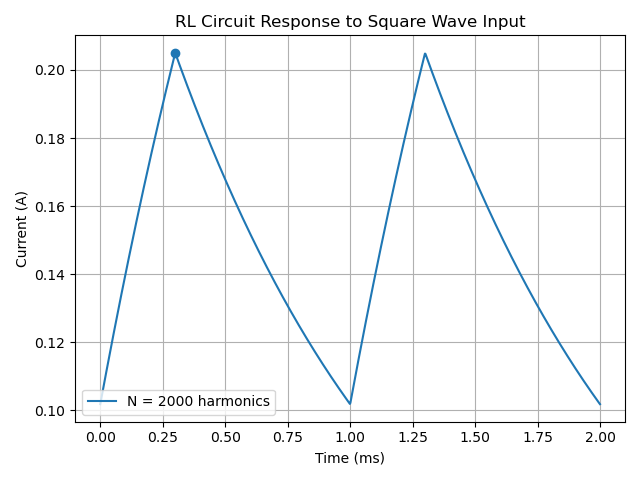
\includegraphics[width=0.8\linewidth]{figs/steady-state.png}
        \caption{Steady state solution to our differential equation}
    \end{figure}
\section{Conclusions}
    The similarity of the solution to a triangular wave is to be expected due to the following fact, 
    \begin{align*}
        \frac{d}{dt}\brak{\text{triangular wave}} = \text{square wave}
    \end{align*}
    In our differential equation as $R \rightarrow 0$, we get,
    \begin{align*}
        \frac{di}{dt} = \frac{V\brak{t}}{L}
    \end{align*}
    which validates our observation.
    \newline
    Coming to the peak deviations from the DC component of the response, the peaks are always located at $t = nT + \alpha T$. So
    \begin{align*}
        \Delta I_o &= \left \|\sum \brak{\frac{A}{n\pi}\frac{\sin\brak{n\pi\alpha}}{R + {jn\omega L}}e^{-jn\pi\alpha}}e^{jn\omega \alpha T} \right\|\\
        &=  \left\| \sum\brak{\frac{A}{n\pi}\frac{\sin\brak{n\pi\alpha}}{R + {jn\omega L}}e^{jn\pi\alpha}} \right \| \\
    \end{align*}
    It is not clear on initial inspection what this series will converge to. So we seek a simpler method to get these offset values.
    \subsection{A simpler way}
    We notice that for system to attain steady state, the current at the starting and end of each cycle should be the same.
    Suppose $I_{cy}$ is the current at the beginning of a cycle in steady state. The inductor will charge through the resistor for time $\Delta t = \alpha T$. So the current at the end of $\alpha T$ seconds will be,
    \begin{align*}
        I_{\alpha T} = \frac{A}{R} + \brak{I_{cy} - \frac{A}{R}}e^{\frac{-R\alpha T}{L}}
    \end{align*}
    For the remainder of the cycle, the inductor discharges. Thus, the current at the end of the cycle is,
    \begin{align*}
        I_{cy}^{\prime} = I_{\alpha T}e^{\frac{-R\brak{T-\alpha T}}{L}}\\
    \end{align*}
    But,
    \begin{align*}
        I_{cy} = I_{cy}^\prime 
    \end{align*}
    On simplification, 
    \begin{align*}
        I_{cy} = \frac{A}{R}e^{\frac{-RT}{L}}\brak{\frac{e^{\frac{R\alpha T}{L}} - 1}{1-e^{\frac{-RT}{L}}}}
    \end{align*}

    From this we calculate the maximum offset to be,
    \begin{align*}
       \Delta I_{max} &= \frac{A}{R} + \brak{I_{cy} - \frac{A}{R}}e^{\frac{-R\alpha T}{L}} - I_{cy}\\
        &= \frac{A}{R}\brak{1 - e^{\frac{-R\alpha T}{L}}} + I_{cy}\brak{e^{\frac{-R\alpha T}{L}} - 1} \\
        &= \brak{1 - e^{\frac{-R\alpha T}{L}}}\brak{\frac{A}{R} - I_{cy}}\\
        &=\frac{A}{R}\brak{1 - e^{\frac{-R\alpha T}{L}}}\brak{1 - \brak{\frac{e^{\frac{R\alpha T}{L}} - 1}{e^{\frac{RT}{L}} - 1}}}\\
        \Delta I_{max} &=\frac{A}{R}\brak{1 - e^{\frac{-R\alpha T}{L}}} \brak{\frac{e^{\frac{RT}{L}}-e^{\frac{R\alpha T}{L}}}{e^{\frac{RT}{L}} - 1}}\\
    \end{align*}

    No wonder we could not find a closed solution previously!\\
    \quad\newline
    So the dependence of the amplitude of oscillation about mean value can be summarized in the following way,
    \begin{enumerate}
        \item Increasing the time period will increase the amplitude of deviations.
        \item Increasing the duty ratio upto 0.5 also increases and after that, it will decrease .
        \item Increasing either the resistance or the inductance will reduce the amplitude of the deviations.
    \end{enumerate}
    \begin{figure}
        \centering
        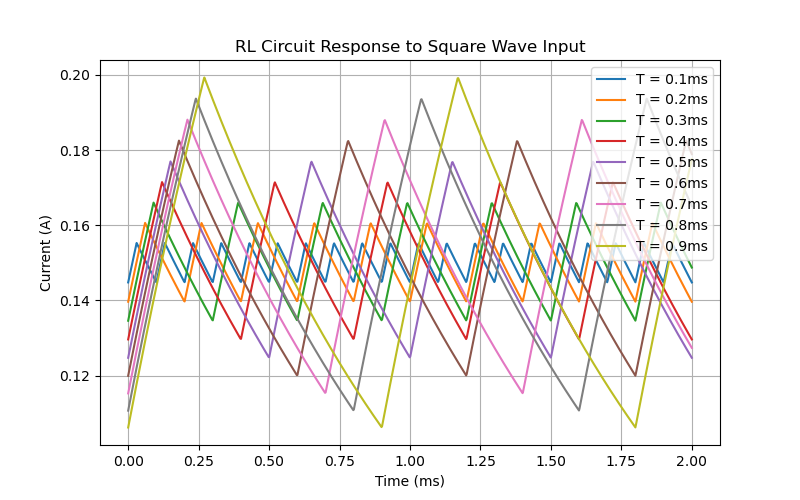
\includegraphics[width=0.8\linewidth]{figs/time-period_variation.png}
        \caption{Variation of amplitude of oscillations with time period}
        \label{fig:enter-label}
    \end{figure}
    \begin{figure}
        \centering
        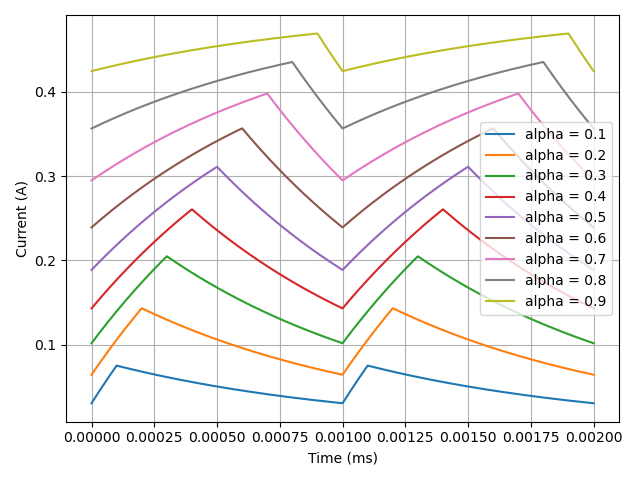
\includegraphics[width=0.8\linewidth]{figs/alpha_variation.png}
        \caption{Variation of amplitude of oscillations with duty ratio}
        \label{fig:enter-label}
    \end{figure}